\section{Umgang mit Daten}
Ein grosses Feature von WPF ist das DataBinding. 
\paragraph{Markup Extensions}
\begin{itemize}
\item \verb+{x:Type [Datentyp]}+: Liefert angegebene Klasse
\item \verb+{x:Static [Pfade]}+: Bindet eine Konstante, statische Property, Feld oder Enum
\item \verb+{x:Null}+: Null Wert
\item \verb+{StaticResource [Name]}+: Statische Bindung an Ressource
\item \verb+{DynamicResource [Name]}+: Dynamische Bindung an Ressource
\item \verb+{Binding ...}+: Data Binding Ausdruck
\item \verb+{RelativeSource ... }+: Setzt die Data Binding Source auf eine relevanten Bezug im Logical Tree
\item \verb+{TemplateBinding ...}+: Bindet Wert an Eigenschaft des mittels Template dargestellten Controls
\item \verb+{x:Reference ...}+: Abk. für \verb+{Binding Elementname=...}+
\end{itemize}
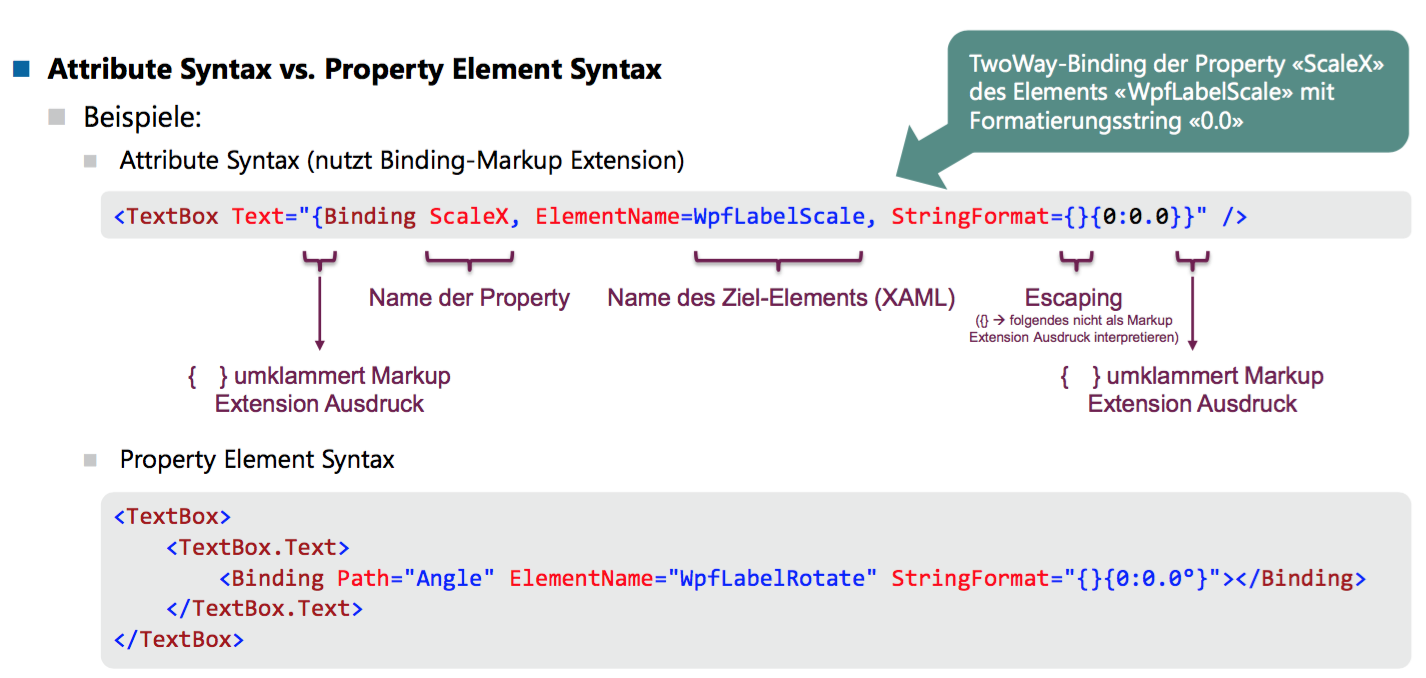
\includegraphics[scale=0.25]{DataBinding.png}
\subsection{Überblick DataBinding}
\paragraph{Binding Base}
\begin{itemize}
\item \verb+Delay+: Verzögerung in Millisekunden zwischen DataBinding Operation
\item \verb+FallbackValue+: Standardwert, falls Data Binding nicht funktioniert
\item \verb+StringFormat+: Formatierungsangabe für die Umwandlung des Quellwertes in einen String
\item \verb+TargetNullValue+: Standardwert, falls Quellwert == null
\end{itemize}
\paragraph{Binding}
\begin{itemize}
    \item \verb+BindsDirectlyToSource+: Soll Angabe der Path-Property relativ zum aktuellen Datenprovider (\verb+true+) oder relativ zum Datenkontext (\verb+false+) ausgewertet werden (Nur selten sinnvoll)
    \item \verb+Converter+: Converter der beim Binding benutzt werden soll
    \item \verb+ConverterCulture+: Länderspezifische Einstellungen (\verb+CultureInfo+), welche beim Konvertieren benutzt werden soll
    \item \verb+ConverterParameter+: Zusätzlicher Parameterwert, der dem Converter übergeben werden soll
    \item \verb+ElementName+: Name des XAML-Elements auf welches gebunden werden soll
    \item \verb+Mode+: Richtung des DataBinding (OneTime, OneWay, TwoWay, OneWayToSource)
    \item \verb+Path+: Pfad zur Datenquelle, Objektpfadsyntax
    \item \verb+XPath+: XPath Ausdruck zum Zugriff auf eine XML Datenquelle
    \item \verb+RelativeSource+: Setzt Datenquelle auf Objekt relative zum Ort des aktuellen Elements
    \item \verb+Source+: Setzt Datenquelle
    \item \verb+UpdateSourceTrigger+: Zeitpunkt zu welchem DataBinding getriggert wird
        \subitem Default: Nutzt festgelegte Trigger der Ziel Property
        \subitem Explicit: Nur beim expliziten Aufruf von \verb+UpdateSource()+
        \subitem LostFocus: Fokusverlust des Elements
        \subitem PropertyChanged: Bei jeder änderung des Inhalts
\end{itemize}

\subsection{DataContext, Source, RelativeSource}
Die Datenquelle ist standartmässig nicht gesetzt, muss also explizit gesetzt werden. 
\paragraph{DataContext} Jedes Element, das von \verb+FrameworkElement+ ableitet, besitzt diese Property. Diese wird Standartmässig von DataBinding als Quelle genutzt und ist ebenfalls in Child-Controls gültig. Diese Property wird im Code-Behind, meist auf Ebene der Fenster, gesetzt.
\paragraph{Source} Ermöglicht die Angabe der Datenquelle direkt im DataBinding Ausdruck. Dieses Property kann auf Ressourcen (Static/Dynamic) oder statische (Static) binden.
\paragraph{RelativeSource} Ermöglicht die Angabe einer relativen Datenquelle im Visual Tree. Es gibt eine eigene Markup Extension dafür. Mit dem Property \verb+Mode+ gibt man den Suchmodus an. Modi dafür sind: \verb+FindAncestor+(Sucht übergeordnetes Element des Typs), \verb+PreviousData+ (Bindet auf das vorhergehende Element, bsp: Delta Vergleiche), \verb+Self+ (Bindet auf das Element selbst), \verb+TemplatedParent+ (Bindet auf Element, für welches Control Template gilt, sinnvoll innerhalb Template). Das Property \verb+AncestorLevel+ Gibt die Vorgänger-Position an und der \verb+AncestorType+ ist der Typ des zu suchenden Vorgänger-Elements.
\begin{lstlisting}[language=xml]
<Label Content="{Binding RelativeSource={RelativeSource FindAncestor, AncestorType=Window}, Path=Title}" />
\end{lstlisting}
\paragraph{Path} Ist die Standart-Property eines Binding-Ausdrucks. Dieser kann deshalb weggelassen werden (\verb+{Binding Firstname}+ ist dasselbe wie \verb+{Binding Path=Firstname}+). Für die Angabe der zu bindenden Property kann auch Objektsyntax verwendet werden (auch Array Syntax ist erlaubt).
\subsection{Converter}
\paragraph{IValueConverter} Ein Interface welches alle Converter implementieren müssen
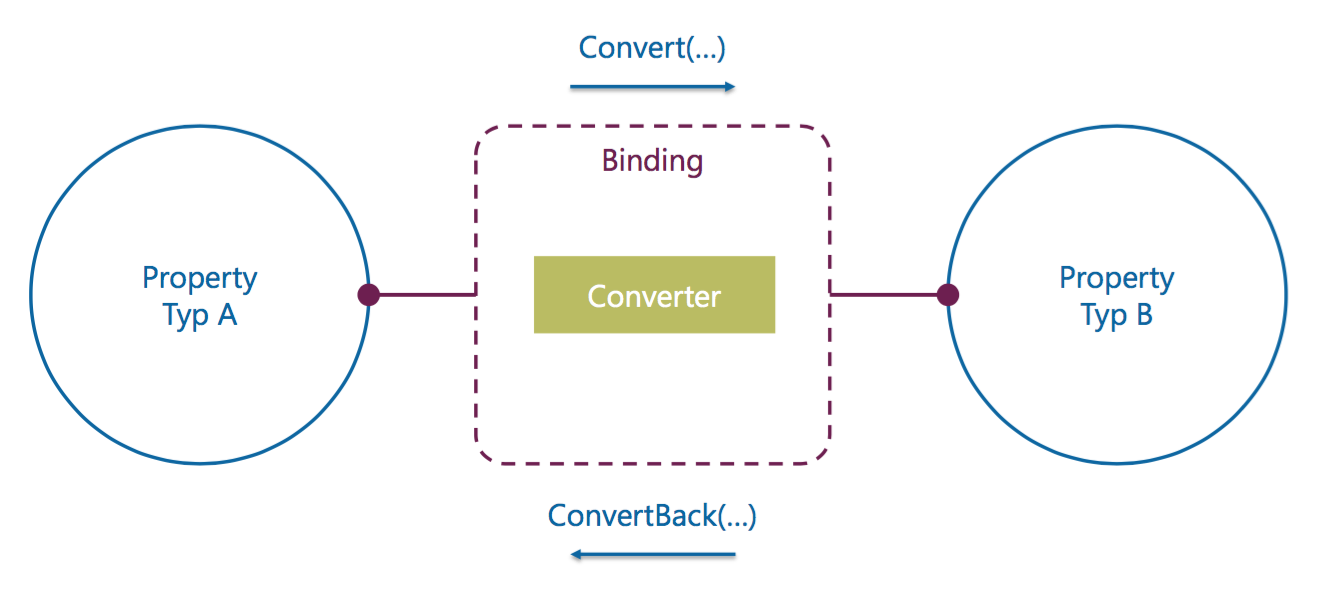
\includegraphics[scale=0.25]{IValueConverter.png}

Es ist auch möglich, nur eine der Methoden zu überschreiben und die andere mit NotImplementedException auszustatten, wenn man es selber nicht verwendet

\begin{lstlisting}[caption="Konvertiert bool oder Nullable in Visibility und zurück"]
public sealed class BooleanToVisibilityConverter: IValueConverter
{
    // value = bool oder nullable, targetType = Visibility
    public object Convert(object value, Type targetType, object parameter, CultureInfo culture)
    {
        return value is bool && (bool)value == true ? Visibility.Visible : Visibility.Collapsed;
    }
    // value = Visibility value, targetType = bool
    public object ConvertBack(object value, Type targetType, object parameter, CultureInfo culture)
    {
        return value as Visibility? == Visibility.Visible
    }
}
\end{lstlisting}
\paragraph{IMultiValueConverter} Das Interface dass alle MultiConverter implementieren müssen.
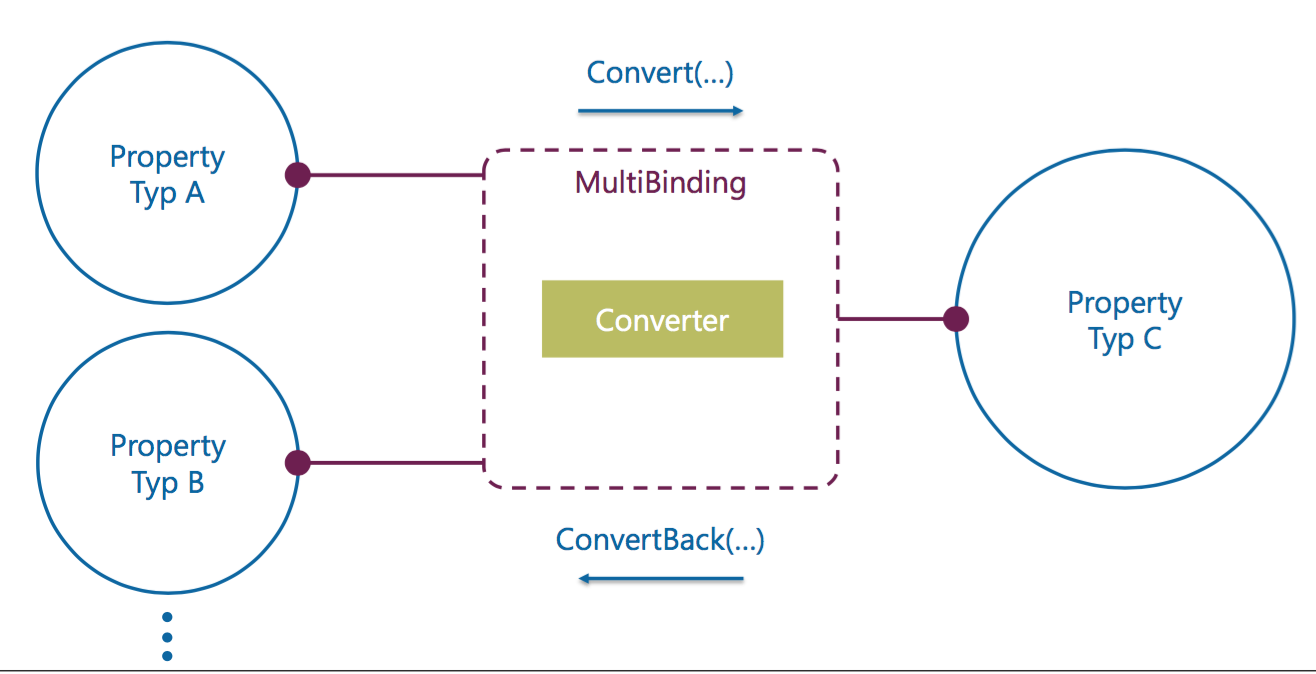
\includegraphics[scale=0.25]{IMultiValueConverter.png}
\begin{lstlisting}
public class RgbToColorConverter: IMultiValueConverter
{
    public object Convert(object[] values, Type targetType, object paramter, CultureInfo culture)
    {
        if (values == null)
            return DependencyProperties.Unsetvalue;
        if(values.Length != 3)
            throw new NotSupportedException("3 Values needed)";
        var r = (byte)System.Convert.ToInt32(values[0]);
        var g = (byte)System.Convert.ToInt32(values[1]);
        var b = (byte)System.Convert.ToInt32(values[2]);
        return Color.FromRgb(r,g,b);
    }
    public object[] ConvertBack(object value, Type[] targetType, object parameter, CultureInfo culture)
    {
        if(value == DependencyProperty.UnsetValue)
            return null;
        if(value is Color)
        {
            var color = (Color) value;
            var colors = new object[] {color.R, color.G, color.B};
            return colors;
        }
        return null;
    }
}
\end{lstlisting}
\paragraph{Value Converter anwenden} Um einen Converter anwenden zu können wird eine Instanz benötigt. Instanziierung:
\begin{lstlisting}[language=xml, caption="Instanzieren"]
<Window.Resources>
    <local:RgbToColorConverter x:Key="MyRgbToColorConverter" />
    <local:BestContrastingColorConverter x:Key="MyBestContrastingColorConverter" />
</Window.Resources>
\end{lstlisting}
Danach kann man den Converter wie gewohnt nutzen:
\begin{lstlisting}
<SolidColorBrush>
    <SolidColorBrush.Color>
        <MultiBinding Converter="{StaticResource MyRgbToColorConverter}">
            <Binding ElementName="ColorR" Path="Value"></Binding>
            <Binding ElementName="ColorG" Path="Value"></Binding>
            <Binding ElementName="ColorB" Path="Value"></Binding>
        </MultiBinding>
    </SolidColorBrush.Color>
</SolidColorBrush>
<SolidColorBrush Color="{Binding Path=Content, ElementName=ColorLabel,
    Converter={StaticResource MyBestContrastingColorConverter}, Mode=OneWay}" />
\end{lstlisting}
Wenn man eigene Value Converters implementiert wird der XAML Code kürzer und man hat eine Entkopplung von Wert und dessen Darstellungseigenschaften. Aber es ist aufwändig und teilweise nicht trivial.
\paragraph{Bindung auf eigene Objekte} Die sogenannten \textbf{DependencyProperties} ermöglichen ein Two-Way Binding und funktionieren mit Key-Value Dictionaries.Sie sind spezialisiert für die Vewendung in einem UI und somit nicht geeignet für Business Objects.
\begin{lstlisting}
public int MyProperty
{
  get {return (int(GetValue(MyPropertyPropert); }
  set { SetValue(MyPropertyProperty, value); }
}
public static readonly DependencyProperty MyPropertyProperty = 
    DependencyPropery.Register("MyProperty", 
            typeof(int), 
            typeoof(ownerclass), 
            new PropertyMetadata(0));
\end{lstlisting}
Mit dem \verb+INotifyPropertyChanged+ Interface können Properties einer Klasse überwacht werden. Das Interface schreibt das Event \verb+PropertyChanged+ vor, das implementiert werden muss. Der Event Handler übermittelt den Namen der geänderten Property.
\begin{lstlisting}
public class Person: INotifyPropertyChanged
{
    private string _firstName;
    public String FirstName
    {
        get {return _firstName; }
        set
        {
            if(value != _firstName)
            {
                _firstName = value;
                OnPropertyChanged(nameof(FirstName));
            }
        }
    }
    public event PropertyChangedeventHandler PropertyChanged;
    public void OnPropertyChanged(string name)
    {
        var handler = PropertyChanged;
        if (handler != null)
            handler(this, new PropertyChangedEventArgs(name));
    }
}
\end{lstlisting}
Dies kann auch mit einer Basisklasse gelöst werden, welche die Benachrichtigung implementiert.
\begin{lstlisting}
public abstract class BindableBase: INotifyPropertyChanged
{
    public event PropertyChangedEventHandler PropertyChanged;
    protected bool SetProperty<T>(ref T field, T value, string name = null)
    {
        if(Equals(field,value))
            return false;
        field=value;
        OnPropertyChanged(name);
        return true;
    }
    protected void OnPropertyChanged(string name = null)
    {
        PropertyChanged?.Invoke(this, new PropertyChangedEventArgs(name));
    }
}
public class Person: BindableBase
{
    private string _firstName;
    public string FirstName;
    {
        get { return _firstName; }
        set { SetProperty(ref _firstName, value, nameof(FirstName)); }
    }
}
\end{lstlisting}
\paragraph{Berechnete Properties} Möchte man Änderungen kommunizieren, sobald sich Quellwerte verändern, muss bei jedem Wechsel eine eigene Notification versendet werden. 
\begin{lstlisting}
protected bool SetProperty<T>(ref T storage, T value, string name, params string[] otherNames)
{
    if(Equals(storage, value))
        return false;
    storage = value;
    OnPropertyChanged(name);
    foreach(var n in otherNames)
        OnPropertyChanged(n);
    return true;
}
\end{lstlisting}

Um das dann zu verwenden, gibt man im Aufruf von SetProperty einfach die berechneten Properties auch noch an, also:
\begin{lstlisting}
private string _lastName;
public string LastName
{
    get { return _lastName; }
    set
    {
        SetProperty(ref _lastName, value, nameof(LastName), 
        nameof(FullName) /*, weitere */);
    }
}
\end{lstlisting}
\paragraph{PropertyChanged.Fody} Fody ist ein Framwork, welches sich in den Kompilationsprozess einhängt und automatisch Properties überwacht. Damit Fody weiss welche Properties er überwachen muss, muss man es mit dem Attribut \verb+ImplementPropertyChanged+ markieren. 
\paragraph{ObservableCollection} Diese Klasse implementiert das INotifyCollectionChanged und INotifyPropertyChanged Interface. Diese Collection meldet Änderungen an sich automatisch, somit ist Event Handling auf neue Listeninhalte, bestimmte Positionen oder die gesamte Liste möglich.
\paragraph{ObjectDataProvider} Ermöglicht Verwendung einer beliebigen Datenquelle mit folgenden Zusatzmöglichkeiten. Es können Parameter an den Konstruktor übergeben werden (ConstructorParameters) oder es können Methoden inkl. Paramter gebunden werden (MethodParameters). Man kann damit beispielsweise Enums auf eine ComboBox binden.
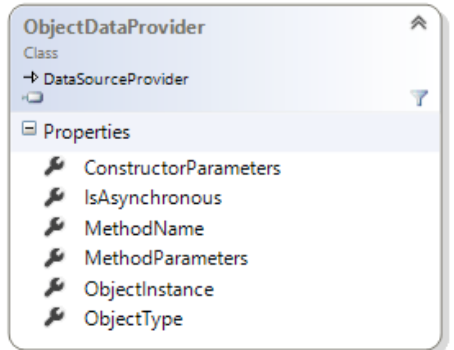
\includegraphics[scale=0.35]{ObjectDataProvider.png}
\begin{lstlisting}[language=xml]
<Window.Resources>
    <ObjectDataProvider x:Key="Alignments"
        MethodName="GetNames"
        ObjectType="{x:Type sys:Enum}">
    <ObjectDataProvider.MethodParameters>
        <x:Type TypeName="VerticalAlignment" />
    </ObjectDataProvider.MethodParameters>
    </ObjectDataProvider>
</Window.Resources>
<!-- Verwendung -->
<ComboBox ItemsSource="{Binding Source={StaticResource Alignments}}" />
\end{lstlisting}
\paragraph{DataBinding Debuggen} Man hat diverse Möglichkeiten die Abläufe hinter dem DataBinding sichtbar zu machen.
\begin{enumerate}
\item Direkt im Binding konfigurieren
\begin{lstlisting}[language=xml]
<!-- System.Diagnostics-Namespace - hinzufuegen -->
xmlns:diag="clr-namespace:System.Diagnostics;assembly=WindowsBase"
<!-- Binding Ausdruck um Setzten des TraceLevels erweitern -->
<TextBlock Text="{Binding ElementName=stack, Path=InvalidPath, diag:PresentationTraceSources.TraceLevel=High}" />
\end{lstlisting}
\item Dummy Converter schreiben
\begin{lstlisting}
public class DebugDummyConverter : IValueConverter
{
    public object Convert(object value, Type targetType, object parameter, CultureInfo culture)
    {
        return value;
    }
    public object ConvertBack(object value, Type targetType, object parameter, CultureInfo culture)
    {
        return value;
    }
}
\end{lstlisting}
\begin{lstlisting}[language=xml]
<Window.Resources> ... <local:DebugDummyConverter x:Key="MyDummy" /> ... </Window.Resources>
...
<TextBlock Text="{Binding ElementName=stack, Path=InvalidPath, Converter={StaticResource MyDummy}}" />
\end{lstlisting}
\item In VisualStudio DataBinding Debugging auf "{}All"{} setzten und im Output-Window nach \verb+Syste.Windows.Data+ suchen.
\end{enumerate}

\subsection{INotifyPropertyChanged (INPC)}
\begin{itemize}
    \item Benötigt bei: \code{OneWay}, \code{TwoWay}
    \item Nicht benötigt bei: \code{OneTime}, \code{OneWayToSource}
\end{itemize}

\subsection{RelayCommand}
''Command-Pattern'', das man selber implementieren muss, aber dann viel Zeit und Geld spart (Ziit und Geld han ich kei).

Nicht-generic RelayCommand
\begin{lstlisting}
public class RelayCommand : ICommand
{
    private readonly Action _execute;
    private readonly Func<bool> _canExecute;
    
    public RelayCommand(Action execute, Func<bool> 
        canExecute = null)
    {
        if (execute == null) throw new 
            ArgumentNullException("execute");
        
        _execute = execute;
        _canExecute = canExecute;
    }
    
    public bool CanExecute(object parameter) => 
        _canExecute?.Invoke() ?? True
    public void Execute(object parameter) => _execute();
    
    // Event an CommandManager delegieren (Benachrichtigung erfolgt
    // so immer dann wenn WPF denkt, dass sich etwas am Ausführungs- 
    // status geändert hat, z.B. bei Key- oder Mouse-Button-Klick)
    public event EventHandler CanExecuteChanged
    {
        add { CommandManager.RequerySuggested += value; }
        remove { CommandManager.RequerySuggested += value }
    }
}
\end{lstlisting}

Die Generic-Variante nutzt ein \mintinline{csharp}{Action<T>} als \mintinline{csharp}{_execute} und ein \mintinline{csharp}{Predicate<T>} als \mintinline{csharp}{_canExecute}

Verwendung:

\begin{lstlisting}
public class GadgetVm : BindableBase
{
    public ICommand SaveCommand { get; set; }
    
    public GadgetVm()
    {
        SaveCommand = new RelayCommand(
            () => this.Save(), // Methode des ViewModels
            () => this.CanSave // Property des ViewModels
        );
    }
    
    public CanSave => ; // some condition
    public void Save() {} // some method
}
\end{lstlisting}

\subsection{Multibinding}
''The new iPhone -- now only 799.00!''. Einleitendes \code{{}} wichtig!

\begin{lstlisting}
<TextBlock>
    <TextBlock.Text>
        <MultiBinding StringFormat="{}{0} -- Now only {1:0.00}!">
            <Binding Path="Description" />
            <Binding ElementName="FirstName" Path="Text" />
        </Multibinding>
    </TextBlock.Text>
</TextBlock>
\end{lstlisting}

\subsection{Binding an anderes Element (Binding Path)}
Mit diesem Code kann man den Inhalt von, z.B. einem TextBlock, an die Eingaben in, z.B. einer Textbox, binden. In diesem Beispiel machen wir dies gleich noch durch ein MultiBinding, der Binding-Ausdruck an sich ist aber allgemeingültig.

\begin{lstlisting}
<TextBox Name="FirstName" />
<TextBox Name="LastName" />
<TextBlock>
    <!-- Anzeige: "FirstName LastName" -->
    <MultiBinding StringFormat="{}{0} {1}">
        <!-- Binden an FirstName.Text -->
        <Binding ElementName="FirstName" Path="Text" />
        <Binding ElementName="LastName" Path="Text" />
    </MultiBinding>
</TextBlock>
\end{lstlisting}